\section{\textcolor{blue}{Tipos de pauta}}
\label{sec:tipospauta}

%%%%%%%%%%%%%%%%%%%%%%%%%%%%%%%%%%%%%%%%%%%%%%%%%%%%%%%%%%%%%%%%%%%%%%%%%%%%%%%%
%%%%%%%%%%%%%%%%%%%%%%%%%%%%%%%%%%%%%%%%%%%%%%%%%%%%%%%%%%%%%%%%%%%%%%%%%%%%%%%%
\subsection{Pauta ou Pentagrama}\index{Pauta}
\label{sec:pauta}
A pauta está representada por 5 linhas paralelas e horizontais, 
as figuras musicais podem ocupar as linhas ou um lugar médio, entre elas.
Adicionalmente, lugares fora da pauta podem ser usados; 
para este proposito, linhas adicionais e parcialmente desenhadas, serão colocadas \cite[pp. 10]{cardoso1973curso}
como é mostrado na Figura \ref{fig:abc-pauta5}.
\begin{figure}[H]
\centering
\begin{abc}[name=abc-pauta5]
% abcm2ps pauta5.abc  -O pauta5.ps
% ps2epsi pauta5.ps pauta5.eps
%
X: 1 % start of header
K: none stafflines=5 %K: C %% Escala de C mayor %
M: none % M: 2/4
%T: Contratempo num compasso binário
V:1 clef=none stem=up name="Pauta"   sname="Pauta"
%
[V:1] C8 D8 E8 F8 G8 A8 B8 C'8 D'8 E'8 F'8 G'8 A'8
\end{abc}
\caption{Pauta com 5 linhas e figuras musicais mostrando algumas posições usáveis.}
\label{fig:abc-pauta5}
\end{figure}
A ordem de leitura das figuras musicais na pauta é de esquerda a direita,
e indica o avanço  do tempo;
as posições das linhas indicam um ordem crescente na altura do som que representam as figuras,
contando desde a linha inferior ate a superior. Nesse sentido, 
uma pauta é semelhante a um espectrograma, onde o eixo X representa o tempo,
o eixo Y representa a frequência, e a figuras colocadas em distintas posições do plano XY, descrevem
o comportamento do sonido nesses dois âmbitos. Assim, a Figura \ref{fig:abc-pauta5}
representa um conjunto de 13 sonidos, cada um com a mesma duração; 
porem, executado com diferentes alturas e em ordem crescente, 
desde um sonido grave ate um sonido mais agudo.
\begin{remark}
As linhas da pauta se contam de abaixo para acima.
As figuras musicais, se leem de esquerda direita, para que corresponda com o sentido do avanço do tempo.
\end{remark}


Por outro lado, se as figuras musicais podem ocupar varias posições entre as linhas da pauta,
pois estos lugares representam alturas diferentes do som; então, 
os silêncios não precisam desta característica,
pelo qual os símbolos que representam os silêncios tem uma posição fixa na pauta,
como pode ser visto na Figura \ref{fig:abc-pautasilencio}.
\begin{figure}[h]
\centering
\begin{abc}[name=abc-pautasilencio]
% abcm2ps pautasilencio.abc  -O pautasilencio.ps
% ps2epsi pautasilencio.ps pautasilencio.eps
%
X: 1 % start of header
K: none stafflines=5 %K: C %% Escala de C mayor %
M: none % M: 2/4
%T: Contratempo num compasso binário
V:1 clef=none name="Pauta"   sname="Pauta"
%
[V:1] z8 z4 z2 z1 z/2 z/4 G8 A4 B2 C'1 D'/2 E'/4 
\end{abc}
\caption{Pauta com 5 linhas e silêncios musicais mostrando algumas posições usáveis.}
\label{fig:abc-pautasilencio}
\end{figure}

O ponto mais interessante, é ver a diferencia do uso  da pausa de mínima e da pausa de semibreve,
dado que estes dois tipos de pausa usam o mesmo símbolo, porem em distintas posições.
Na Figura \ref{fig:abc-pautasilencio} a pausa de semibreve, 
está colocada em primeiro lugar desde a esquerda da pauta,
e o símbolo está desenhado unido a parte baixa de uma linha da pauta.
Por outro lado, a pausa de mínima está desenhada no segundo lugar da pauta,
contando desde a esquerda, e se desenha unida à parte de acima de uma linha da pauta.
Estos dois simbolo podem estar desenhados em duas linhas diferentes, 
como no exemplo da Figura \ref{fig:abc-pautasilencio}, ou na mesma linha.

\subsubsection{As claves na pauta}
\label{subsubsec:clavespauta}
A clave, como símbolo, 
se coloca ao inicio da pauta, 
e serve para indicar as alturas das notas na pauta \cite[pp. 179]{apel1969harvard} \cite[pp. 10]{cardoso1973curso}.
Existem 3 tipos de claves\footnote{E varias posições para estas, porem aqui veremos as mas basicas.} que podem ser usadas na pauta, 
assim temos: 
\begin{description}
\item [Clave sol:] Representada pelo símbolo 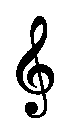
\includegraphics[height=14pt]{chapters/cap-musica-basica/G-clef.eps}. 
A posição donde esta clave se assine indica o lugar onde se localiza uma nota sol.
\begin{example}
Na Figura \ref{fig:abc-clavesol} podemos ver à clave de sol assinada sobre a segunda linha da pauta,
indicando que esta linha representa a nota sol.
\end{example} 
\item [Clave de fá:] Representada pelo símbolo 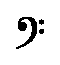
\includegraphics[height=10pt]{chapters/cap-musica-basica/FClef.eps}. 
A posição donde essa clave se assine indica o lugar onde se localiza uma nota fá.
\begin{example}
Na Figura \ref{fig:abc-clavefa} podemos ver à clave de fá assinada sobre a quarta linha da pauta,
indicando que essa linha representa a nota fá.
\end{example} 
\item [Clave de dó:] Representada pelo símbolo 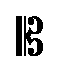
\includegraphics[height=10pt]{chapters/cap-musica-basica/CClef.eps}.
A posição donde esta clave se assine indica o lugar onde se localiza uma nota dó.
\begin{example}
Na Figura \ref{fig:abc-clavedo} podemos ver à clave de dó assinada sobre a terceira linha da pauta,
indicando que essa linha representa a nota dó.
\end{example} 
\end{description}
%%%
\begin{figure}[h]
    \centering
\begin{subfigure}[c]{0.25\textwidth}
\begin{abc}[name=abc-clavesol]
% abcm2ps clavesol.abc  -O clavesol.ps
% ps2epsi clavesol.ps clavesol.eps
%
X: 1 % start of header
K: C stafflines=5 %K: C %% Escala de C mayor %
M: none % M: 2/4
%T: Contratempo num compasso binário
V:1 clef=treble %name="Pauta com clave de sol"   sname="Pauta com clave de sol"
%
[V:1] G8
\end{abc}
\caption{Clave de sol com uma semibreve colocada em sol.}
\label{fig:abc-clavesol}
\end{subfigure}
~ %
\begin{subfigure}[c]{0.25\textwidth}
\begin{abc}[name=abc-clavefa]
% abcm2ps clavesfa.abc  -O clavefa.ps
% ps2epsi clavefa.ps clavefa.eps
%
X: 1 % start of header
K: C stafflines=5 %K: C %% Escala de C mayor %
M: none % M: 2/4
%T: Contratempo num compasso binário
V:1 clef=bass %name="Pauta com clave de fá"   sname="Pauta com clave de fá"
%
[V:1] F,8  
\end{abc}
\caption{Clave de fá com uma semibreve colocada em fá.}
\label{fig:abc-clavefa}
\end{subfigure}
~ %
\begin{subfigure}[c]{0.25\textwidth}
\begin{abc}[name=abc-clavedo]
% abcm2ps clavesfa.abc  -O clavedo.ps
% ps2epsi clavedo.ps clavedo.eps
%
X: 1 % start of header
K: C stafflines=5 %K: C %% Escala de C mayor %
M: none % M: 2/4
%T: Contratempo num compasso binário
V:1 clef=C %name="Pauta com clave de fá"   sname="Pauta com clave de fá"
%
[V:1] C8 
\end{abc}
\caption{Clave de dó com uma semibreve colocada em dó.}
\label{fig:abc-clavedo}
\end{subfigure}
    \caption{Tipos de claves}\label{fig:allclaves}
\end{figure}



\subsubsection{As claves e a escala diatonica}
Conhecida as definições das claves, e da \hyperref[sec:pos:Diatonica]{\textbf{escala diatônica}}, 
podemos misturar estes dois conceitos para conhecer a posição de todas as notas na pauta
\cite[pp. 10]{cardoso1973curso} \cite[pp. 14]{medteoria}.

Por exemplo, as pautas desenhadas na Figura \ref{fig:allnotesclaves} 
contem duas duas oitavas cada uma, centradas em dó, e com notas escritas usando semibreves.
\begin{figure}[h]
    \centering
\begin{abc}[name=abc-clavenotessol]
% abcm2ps clavenotessol.abc  -O clavenotessol.ps
% ps2epsi clavenotessol.ps clavenotessol.eps
%
X: 1 % start of header
K: C stafflines=5 %K: C %% Escala de C mayor %
M: none % M: 2/4
%T: Contratempo num compasso binário
V:1 clef=treble %name="Pauta com clave de sol"   sname="Pauta com clave de sol"
%
[V:1] "dó"C,8 "ré"D,8 "mi"E,8 "fá"F,8  "sol"G,8 "lá"A,8 "si"B,8 "dó"C8 "ré"D8 "mi"E8 "fá"F8  "sol"G8 "lá"A8 "si"B8 "dó"C'8 
\end{abc}

\begin{abc}[name=abc-clavenotesfa]
% abcm2ps clavenotesfa.abc  -O clavenotesfa.ps
% ps2epsi clavenotesfa.ps clavenotesfa.eps
%
X: 1 % start of header
K: C stafflines=5 %K: C %% Escala de C mayor %
M: none % M: 2/4
%T: Contratempo num compasso binário
V:1 clef=bass %name="Pauta com clave de fá"   sname="Pauta com clave de fá"
%
[V:1] C,8 D,8 E,8 F,8 G,8 A,8 B,8 C8 D8 E8 F8 G8 A8 B8 C'8 
\end{abc}

\begin{abc}[name=abc-clavenotesdo]
% abcm2ps clavenotesfa.abc  -O clavenotesdo.ps
% ps2epsi clavenotesdo.ps clavenotesdo.eps
%
X: 1 % start of header
K: C stafflines=5 %K: C %% Escala de C mayor %
M: none % M: 2/4
%T: Contratempo num compasso binário
V:1 clef=C %name="Pauta com clave de fá"   sname="Pauta com clave de fá"
%
[V:1] C,8 D,8 E,8 F,8 G,8 A,8 B,8 C8 D8 E8 F8 G8 A8 B8 C'8 
\end{abc}
    \caption{Tipos de claves}\label{fig:allnotesclaves}
\end{figure}
Na pauta com clave de sol, 
se distingue como as notas da oitava mais alta estão bem posicionadas na pauta;
porem, as notas da oitava inferior precisam linhas adicionais para serem representadas,
o que dificultará ou não deixará muito elegante a leitura dos elementos na pauta.
Podemos ver um caso similar, pero ao contrario, com a pauta que usa uma clave de fá;
nela, as notas da primeira oitava estão comodamente representadas dentro da pauta;
porem, as da oitava superior precisam linhas adicionais.
Finalmente, a notas escritas usando a clave de dó, estão bem centradas,
para notas com alturas intermédias e só fica fora da pauta as duas notas mais aguda e as duas mais graves.

A primeira vista poderia parecer mais vantajosa a clave de do, 
porem isto acontece só porque a nota central que queremos representar é um dó,
teríamos uma vantagem similar na clave de sol, se usaremos uma nota central em si,
ou a vantagem a teríamos na clave de fá, se usaremos uma nota central em ré. 
Na prática, escolher entre
uma clave u outra dependerá da melodia que queiramos encaixar na pauta.
Porem existe uma combinação muito usada na musica para piano, 
que é usar uma clave de sol pra descrever as melodias a serem tocadas pela mão direita,
e usar uma clave de fá, para as que serão tocadas pela mão esquerda; 
isto é conveniente devido a que se olhamos o dó central nessas claves, 
na Figura \ref{fig:allnotesclaves}, 
poderemos observar que esta nota se sai das linhas da pauta, 
justo para entrar nas linhas da pauta da outra mão.

%%%%%%%%%%%%%%%%%%%%%%%%%%%%%%%%%%%%%%%%%%%%%%%%%%%%%%%%%%%%%%%%%%%%%%%%%%%%%%%%
%%%%%%%%%%%%%%%%%%%%%%%%%%%%%%%%%%%%%%%%%%%%%%%%%%%%%%%%%%%%%%%%%%%%%%%%%%%%%%%%
\subsection{\textcolor{green}{Pauta de percussão}}\index{Pauta!Pauta de Percussão}

Existem varias formas de representar as pautas para percussão, 
estas são diferenciadas do pentagrama, devido a que na percussão, 
na maioria dos casos não se tem controle da \hyperref[sec:pos:Duracion]{\textbf{duração}} do som;
e sim se tem, do momento em que este será executado. Em outros casos,
pode estar desabilitada a possibilidade de mudar a \hyperref[sec:pos:Altura]{\textbf{altura}} dos sons;
pelo que não se necessitam linhas pra representar estas alturas.
Assim, as pautas de percussão estarão optimizadas, em cada caso, 
para mostrar com simplicidade o ritmo que se deseja interpretar.

\subsubsection{A clave de percussão}
Também chamada \textbf{clave neutral} ou \textbf{clave de ritmos}, 
porque é usada por percussionistas, bateristas, 
ou usada para qualquer instrumento que produz um som que não tem uma altura definida \cite[pp. 51]{harnum2009basic}.
Asim, esta clave indica que a pauta mostra ritmos e modos de tocar um instrumento, 
e não indica as alturas das notas, 
como outras claves mostradas na Seção \ref{subsubsec:clavespauta}.
Podemos achar dois símbolos equivalentes para representar esta clave, 
estes são \includegraphics[height=10pt]{chapters/cap-musica-basica/P1-clef.eps}
e \includegraphics[height=10pt]{chapters/cap-musica-basica/P2-clef.eps}.
Entre os instrumentos que usam esta clave temos:
o tambourine, o triangulo, o pandeiro, etc.
A Figura \ref{fig:allpercusionclaves} mostra algumas formas de usar a clave de percussão,
sendo formas equivalentes, as mostradas na Figura \ref{fig:abc-claveperczero} e a Figura \ref{fig:abc-clavepercuma}.

\begin{figure}[h]
    \centering 
\begin{subfigure}[c]{0.24\textwidth}
\begin{abc}[name=abc-clavepercusion1]
% abcm2ps clavepercusion1.abc  -O clavepercusion1.ps
% ps2epsi clavepercusion1.ps clavepercusion1.eps
%
X: 1 % start of header
K: C stafflines=0 %K: C %% Escala de C mayor %
M: none % M: 2/4
%T: Contratempo num compasso binário
V:1 clef=perc stem=up %name="Pauta com clave de fá"   sname="Pauta com clave de fá"
%
[V:1] B1 B1 B2 B1 B2   
\end{abc}
\caption{Clave de percussão sem linhas, indicando que só existe um modo de tocar o instrumento.}
\label{fig:abc-claveperczero}
\end{subfigure}
~%
\begin{subfigure}[c]{0.24\textwidth}
\begin{abc}[name=abc-clavepercusion2a]
% abcm2ps clavepercusion2a.abc  -O clavepercusion2a.ps
% ps2epsi clavepercusion2a.ps clavepercusion2a.eps
%
X: 1 % start of header
K: C stafflines=1 %K: C %% Escala de C mayor %
M: none % M: 2/4
%T: Contratempo num compasso binário
V:1 clef=perc stem=up %name="Pauta com clave de fá"   sname="Pauta com clave de fá"
%
[V:1] B1 B1 B2 B1 B2   
\end{abc}
\caption{Clave de percussão com uma linha e só um modo de tocar o instrumento.}
\label{fig:abc-clavepercuma}
\end{subfigure}
~%
\begin{subfigure}[c]{0.24\textwidth}
\begin{abc}[name=abc-clavepercusion2]
% abcm2ps clavepercusion2.abc  -O clavepercusion2.ps
% ps2epsi clavepercusion2.ps clavepercusion2.eps
%
X: 1 % start of header
K: C stafflines=1 %K: C %% Escala de C mayor %
M: none % M: 2/4
%T: Contratempo num compasso binário
V:1 clef=perc stem=up %name="Pauta com clave de fá"   sname="Pauta com clave de fá"
%
[V:1] A1 C'1 A2 C'1 A2   
\end{abc}
\caption{Clave de percussão com uma linha e dois modos de tocar o instrumento.}
\label{fig:abc-clavepercum2}
\end{subfigure}
~%
\begin{subfigure}[c]{0.24\textwidth}
\begin{abc}[name=abc-clavepercusion3]
% abcm2ps clavepercusion3.abc  -O clavepercusion3.ps
% ps2epsi clavepercusion3.ps clavepercusion3.eps
%
X: 1 % start of header
K: C stafflines=5 %K: C %% Escala de C mayor %
M: none % M: 2/4
%T: Contratempo num compasso binário
V:1 clef=perc stem=up %name="Pauta com clave de fá"   sname="Pauta com clave de fá"
%
[V:1] A1 B1 G2 C'1 F2   
\end{abc}
\caption{Clave de percussão com cinco linhas e vários modos de tocar o instrumento.}
\label{fig:abc-claveperccinco}
\end{subfigure}
    \caption{Usos da clave de percussão}\label{fig:allpercusionclaves}
\end{figure}

\subsubsection{O sistema de notação monolinear}
Este sistema foi criado pelo baterista suiço, Dr. Fritz Berger, em 1928. 
Ele o chamou ``the monolinear notation system'', 
de modo que seu sistema utilizava uma única linha na pauta, na sua definição,
a parte de acima da linha representava a mão direita (para bateria), e
a parte de abaixo da linha a mão esquerda.
Assim, era mais fácil ler os ritmos, deixando claro que mão devia fazer uma determinada ação
\cite[pp. 148]{beck1995encyclopedia} \cite[pp. 332]{dean2012drum}.
Um exemplo deste sistema pode ser visto na Figura \ref{fig:abc-clavepercum2}.

\subsubsection{The grid notation}


\cite[pp. 289]{gould676behind}

\begin{comment}
\subsubsection{The musical notation of percusion}
Revisar  \cite[pp. 70]{harnum2009basic}

Figura \ref{fig:abc-musicalperc}
\begin{figure}[H]
\centering
\begin{abc}[name=abc-musicalperc]
% abcm2ps musicalperc.abc  -O musicalperc.ps
% ps2epsi musicalperc.ps musicalperc.eps
%
X:1
T:Drum Key
M:
L:1/4
K:C clef=perc
"^Bass"F|"^Snare"c|"^High tom"e|"^Mid tom"d|"^Low tom"B|"^Floor tom"A|
"^Cymbal"^b|"^Crash"^a|"^Hi-hat"^g|"^Ride"^f|"^Hi-hat Pedal"^D|]

\end{abc}
\caption{Figuras e pausas}
\label{fig:abc-musicalperc}
\end{figure}
\end{comment}


